\section{Mini-Project A}
\label{sec:ProjA}
This project examines ELO5.2, which requires the student to develop a representative embedded system. It requires hardware/software interfacing, so an ADC is sampled by software, and processing operations are applied to read the data. 

\subsection{Pre-Project Requirements}
\begin{itemize}
    \item You will need to have completed all the previous practicals in order to complete this project.
    \item Using the design flows presented in class, we strongly recommend beginning by drawing up an initial design and mapping the required tasks to (at the least) a simple timeline or Gantt chart.
\end{itemize}

\subsection{Outcomes}
In addition to creating a working system, you will learn about the following in this project:
\begin{itemize}
    \item ADC - \href{https://cdn-shop.adafruit.com/datasheets/MCP3008.pdf}{MCP3008}
    \item Temperature sensor - \href{http://ww1.microchip.com/downloads/en/devicedoc/20001942g.pdf}{MCP9700A}
    \item IOT - \href{https://blynk.io/}{Blynk}
\end{itemize}

\subsection{Deliverables}
At the end of this practical, you must:
\begin{itemize}
    \item Demonstrate your working implementation to a tutor through a formal presentation. This will take the form of a formal presentation in a 10 minute slot you will book in advance. See Table \ref{tbl:DemoValidation} for details on the demonstration.
    \item Submit your report to Vula, in the format shown in Table \ref{tbl:flamarks}
    \item For information on the marks and what sections to cover, refer to the marking guide in Section \ref{sec:ProjAMarks}
\end{itemize}

\subsection{Hardware Required}
\begin{tabular}{ll}
\begin{tabular}[c]{@{}l@{}}
\tabitem All hardware from previous pracs\\ 
\tabitem Potentiometer to mimic VPD sensor\\ 
\tabitem LDR\\
\end{tabular} 
&\begin{tabular}[c]{@{}l@{}}
\tabitem ADC\\ 
\tabitem Temperature Sensor - to be distributed\\ 
\\
\end{tabular} 
\end{tabular}

\subsection{System Overview}
Figure \ref{fig:SystemOverview} shows the system overview for the mini project.
\begin{figure}[H]
\centering
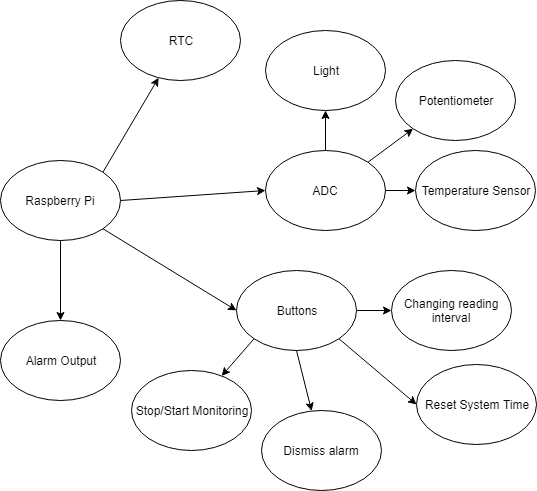
\includegraphics[width=0.8\columnwidth]{Figures/SystemOverview}
\caption{Components of the Mini-Project}
\label{fig:SystemOverview}
\end{figure}

\begin{multicols}{2}
Figure \ref{fig:blynkexample} shows an example of what the app you create in Blynk might look like.
As you can see there's a terminal for accessing the output of the print statements, three values as read from the ADC, and an indicator to indicate if the alarm has gone off. There are various widgets in Blynk. It's suggested you play with your energy budget to develop the most intuitive design and aesthetically pleasing design possible.
\vfill\null
\columnbreak
\begin{figure}[H]
\centering
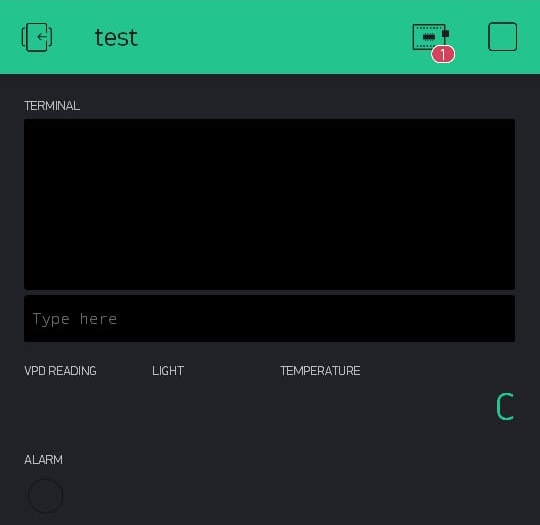
\includegraphics[width=0.75\columnwidth]{Figures/blynkexample}
\caption{Example Blynk Project}
\label{fig:blynkexample}
\end{figure}
\end{multicols}


\subsection{Hardware requirements}
You will need to build your design and demonstrate it to the marker.

\subsection{Software requirements}
You need to do the following:
\begin{itemize}
    \item Set up the RTC using the Raspberry Pi's supplied kernel driver for an RTC
    \item Create a thread for reading from the ADC. The value read from the temperature sensor needs to be converted to degrees Celsius. See the datasheet (linked above) for the formula.
    \item Create interrupts for all the button functionality (don't forget to debounce your inputs)
    \item Output the correctly calculated voltage over the DAC.
    \item Create an output signal to notify the biology student that there is an issue. You can flash an LED using a PWM signal, you can play audio through the audio jack, or you can buy a buzzer from WhiteLab. 
    \item In the main() loop, print values to the screen as described in Section \ref{sec:ProjDescription}
\end{itemize}

\subsection{Description}
\label{sec:ProjDescription}
\begin{itemize}
    \item The system should have hard-coded thresholds. When a value read by the device goes over a threshold, an alarm should sound. A button must be pressed to dismiss the alarm.
    \item By default, the system continuously monitors the sensors every 1s using this format:
    \begin{table}[H]
    \centering
    \begin{tabular}{|l|l|l|l|l|l|l|}
    \hline
    RTC Time & Sys Timer & Humidity  & Temp  & Light & DAC out & Alarm \\ \hline
    10:17:15 & 00:00:00 & 0.5 V &   25 C    & 595 & 0.29V&* \\ \hline
    10:17:20 & 00:00:05 & 1.5 V &   25 C    & 595 & 0.87V&* \\ \hline
    10:17:25 & 00:00:10 & 1.7 V &   25 C    & 595 & 0.98V&  \\ \hline
    10:17:30 & 00:00:15 & 2.2 V &   25 C    & 782 & 1.68V&  \\ \hline
    10:17:35 & 00:00:15 & 3.3 V &   25 C    & 998 & 3.22V&  \\ \hline
    \end{tabular}
    \end{table}
    Notice how the alarm flag is still active at 10:17:20, as it is only dismissed before the reading at 10:17:25. Also note that even though the DAC out value exceeds the alarm threshold at time 10:17:35, no alarm is sounded as the last alarm was sounded less than three minutes prior. 
    \item The reset switch resets the system timer and cleans the console
    \item The frequency switch changes the frequency of the monitoring. The possible frequencies are 1s, 2s and 5s. The frequency must loop between those values per event occurrence.
    \item The stop switch stops or starts the monitoring of the sensors. The system timer is not affected by this functionality.
    \item The display switch displays the first five reading since the stop switch was pressed.
    \item Blynk must be used to:
    \begin{itemize}
        \item View live logging information (System time and ADC values)
        \item Be notified of alarms
    \end{itemize}
\end{itemize}

\subsection{Marking Guide}
\label{sec:ProjAMarks}
\begin{longtable}[c]{|l|l|l|}
\caption{Project A marking Guide}
\label{tbl:flamarks}\\
\hline
\textbf{Heading} & \textbf{Report} & \textbf{Demo} \\ \hline
\endfirsthead
%
\endhead
%
Introduction & \begin{tabular}[c]{@{}l@{}}Provide a short introduction ($\sim \frac{1}{2}$ page)\\ to your project explaining your main\\ design choices and how the report has\\ been structured (15 marks)\end{tabular} & \begin{tabular}[c]{@{}l@{}}Introduce yourselves and\\ your project. {[}8 marks{]}\end{tabular} \\ \hline
Requirements & \begin{tabular}[c]{@{}l@{}}The requirements section should\\ provide a refined UML Use Case\\ diagram of the system, according to\\ your implementation, and any\\ accompanying text that is needed to\\ clarify the requirements.\\ Highlight any departures or additions\\ that you may have made compared to\\ the original project description given in\\ this document. {[}15 marks{]}\end{tabular} & \begin{tabular}[c]{@{}l@{}}Have an (at least draft)\\ UML Use Case to show\\ the tutor. Show this\\ briefly, indicating any\\ departures/additions.\\ {[}6 marks{]}\end{tabular} \\ \hline
\begin{tabular}[c]{@{}l@{}}Specification \\ and Design\end{tabular} & \begin{tabular}[c]{@{}l@{}}This section should provide a UML\\ State Chart describing the main\\ operation. Add a UML class or\\ deployment diagram (or other suitable\\ diagram) to indicate the structuring of\\ your implementation (e.g. code\\ modules/classes you may be using).\\ You don’t need to provide fine detail of\\ the system, the diagram(s) can be e.g.\\ at the level of functions. You should\\also include a circuit diagram {[}20 marks{]}\end{tabular} & \begin{tabular}[c]{@{}l@{}}Briefly show your design,\\ you need not show more\\ than one rough diagram\\ (e.g. draft state chart) to\\ the tutor. {[}10 marks{]}\end{tabular} \\ \hline
Implementation & \begin{tabular}[c]{@{}l@{}}This section should give some snippets\\ of important code and explanations for\\ this (or referring to particular\\ functions in code files). The point here\\ is elaborating any parts of the State\\ Chart that are not so straightforward\\ to turn into code. {[}20 marks{]}\end{tabular} & \begin{tabular}[c]{@{}l@{}}You should have a code\\ file open already (e.g.\\ where the main function\\ is) before you start the\\ demo. Briefly confirm to\\ the tutor that this is part\\ of the program that will be\\ demoed. {[}6 marks{]}\end{tabular} \\ \hline
\begin{tabular}[c]{@{}l@{}}Validation and\\ Performance\end{tabular} & \begin{tabular}[c]{@{}l@{}}Provide at least a paragraph or two\\ explaining the performance of the\\ system. A snapshot could be included\\ and you could show test cases where\\ you have tested that the system works\\ reliably (e.g. using a powersupply to set \\ the value given to the ADC). {[}20\\ marks{]}\end{tabular} & \begin{tabular}[c]{@{}l@{}}This is a main aspect of\\ the demonstration.\\ See Validation Check\\ Sheet in Section \ref{sec:ProjAValidation}.\\ {[}40 marks{]}\end{tabular} \\ \hline
Conclusion & \begin{tabular}[c]{@{}l@{}}Give a summary of the extent that the\\ system was found to be successful.\\ Discuss if you think that a system\\ working in this way might be\\ considered a potentially useful product.\\ {[}10 marks\end{tabular} & \begin{tabular}[c]{@{}l@{}}End you demo with a\\ short conclusion, reflect\\ on the activity. {[}10 marks{]}\end{tabular} \\ \hline
References & Provide a few references if relevant. & Questions {[}20 marks{]} \\ \hline
Total & 100 &  \\ \hline
\end{longtable}

\subsection{Project A Validation Sheet}
\label{sec:ProjAValidation}
% Please add the following required packages to your document preamble:
% \usepackage{graphicx}
\begin{table}[H]
\centering
\caption{The Mark sheet used in Demos}
\label{tbl:DemoValidation}
\resizebox{\textwidth}{!}{%
\begin{tabular}{|l|l|l|r|l|}
\hline
\multicolumn{2}{|l|}{\textbf{Demo Mark Validation Sheet}} & \multicolumn{3}{l|}{Marked by:} \\ \hline
\multicolumn{5}{|l|}{Student Numbers:} \\ \hline
\textbf{Component} & \textbf{Category} & \textbf{Description} & \multicolumn{1}{l|}{\textbf{Max Marks}} & \textbf{Mark} \\ \hline
\textbf{Blynk} & \begin{tabular}[c]{@{}l@{}}Connected \\ and responds\end{tabular} & \begin{tabular}[c]{@{}l@{}}Blynk should connect to the Pi (2) \\ and reponds to changes on the Pi \\ (5 - ldr, pot, temp, alarm, start/stop log)\end{tabular} & 7 &  \\ \hline
 & Design & \begin{tabular}[c]{@{}l@{}}All features of the EnviroLogger should \\ be reflected in the widgets used in Blynk\end{tabular} & 5 &  \\ \hline
 &  & \begin{tabular}[c]{@{}l@{}}The use of widgets should be aesthetically \\ pleasing as well as intuitive (use of labels, \\ placement of widgets)\end{tabular} & 2 &  \\ \hline
\textbf{ADC} & Temperature & \begin{tabular}[c]{@{}l@{}}Temperature reported on is accurate and \\ responds to input (warming up when \\ sensor is held, etc)\end{tabular} & 2 &  \\ \hline
 & Potentiometer & \begin{tabular}[c]{@{}l@{}}Responds to changes input, reading \\ displayed is between 0 and 3.3V\end{tabular} & 2 &  \\ \hline
 & Light sensor & \begin{tabular}[c]{@{}l@{}}Voltage divider with resistor of equal \\ value to LDR\end{tabular} & 2 &  \\ \hline
 &  & Reports a value between 0 and 1023 & 2 &  \\ \hline
\textbf{\begin{tabular}[c]{@{}l@{}}Buttons/\\ Logging\end{tabular}} & Implementation & \begin{tabular}[c]{@{}l@{}}Uses interrupts (1 ea) and \\ debouncing (1 ea)\end{tabular} & 8 &  \\ \hline
 & Interval Reading & Changes between 1, 2 and 5s & 3 &  \\ \hline
 & Reset SysTime & Resets system time to 0 & 1 &  \\ \hline
 & Dismiss Alarm & \begin{tabular}[c]{@{}l@{}}Clears alarm and outputs message \\ saying so.\end{tabular} & 2 &  \\ \hline
 & \begin{tabular}[c]{@{}l@{}}Stop/Start \\ logging\end{tabular} & \begin{tabular}[c]{@{}l@{}}Pauses the print out to system console,\\  but timer continues increasing\end{tabular} & 1 &  \\ \hline
\textbf{Alarm} & Implementation & Calculation implemented & 1 &  \\ \hline
 & DAC & Outputs correct voltage & 1 &  \\ \hline
 & Alarm & \begin{tabular}[c]{@{}l@{}}Can't sound more often than 3 min\\ intervals\end{tabular} & 1 &  \\ \hline
\textbf{Mark} &  &  & \textbf{40} &  \\ \hline
\end{tabular}%
}
\end{table}